\documentclass{scrartcl}

\usepackage{amsmath}
\usepackage{amsthm}
\usepackage{amssymb}
\usepackage[utf8]{inputenc}
\usepackage{amsfonts}
\usepackage{phaistos}
\usepackage{enumerate}
\usepackage{mathtools}
\usepackage[ngerman]{babel}
\usepackage{graphicx}
\usepackage{amsthm}
\usepackage{wasysym}
\usepackage{fontawesome}
\usepackage{marvosym}
\usepackage{pdfpages}
\usepackage{color}
 \usepackage[T1]{fontenc}
 \usepackage{textcomp}
 \usepackage{gensymb}
 \usepackage{newunicodechar}
 \graphicspath{	{./Bilder/}	} 
 \setlength{\parindent}{0em}
 \usepackage[center]{caption}
 \usepackage[normalem]{ulem}
 \usepackage{booktabs} 
 \usepackage{subfig} 
 \usepackage{float}
 \usepackage{xpatch}
 \usepackage[shortlabels]{enumitem}
 \usepackage[textwidth=13cm]{geometry}
 \usepackage[notref,notcite]{showkeys}
 \usepackage{soul}
\usepackage{ mathrsfs }

\newcommand{\oa}{\overline{a}}
\newcommand{\ooa}{\overline{\overline{a}}}
\newcommand{\ob}{\overline{b}}
\newcommand{\dsum}{\displaystyle\sum}
\newcommand{\K}{\mathbb{K}}
\newcommand{\Z}{\mathbb{Z}}
\newcommand{\Q}{\mathbb{Q}}
\newcommand{\R}{\mathbb{R}}
\newcommand{\N}{\mathbb{N}}
\newcommand{\C}{\mathbb{C}}
\newcommand{\M}{M\text{°}}
\newcommand{\calM}{\ensuremath{\mathcal{M}}}
\newcommand{\calMnm}{\ensuremath{\calM_{n\times m}}}
\newcommand{\calMn}{\ensuremath{\calM_{n}}}
\newcommand{\lin}[1]{\ensuremath{\text{lin\ensuremath{\left\{ #1 \right\}}}}}
\newcommand{\Kern}[1]{\ensuremath{\text{Ker}\left(#1\right)}}
\newcommand{\func}[2]{\ensuremath{#1 \left(#2\right)}}
\newcommand{\Bild}[1]{\ensuremath{\text{Bild}\left(#1\right)}}
\newcommand{\rang}[1]{\ensuremath{\text{Rang}\left(#1\right)}}
\newcommand{\F}{\mathbb{F}}
\newcommand{\RN}[1]{\textup{\uppercase\expandafter{\romannumeral#1}}}
\newcommand{\matrx}[1]{\begin{pmatrix}#1\end{pmatrix}}
\newcommand{\set}[1]{\ensuremath{\left\{ #1 \right\}}}
\newcommand{\abs}[1]{\ensuremath{\left\vert #1 \right\vert}}
\newcommand{\dabs}[1]{\ensuremath{\left\vert\left\vert#1\right\vert\right\vert}}
\newcommand{\scp}[1]{\ensuremath{\left<#1\right>}}
\newcommand{\dbcup}[2][]{\ensuremath{\displaystyle\bigcup_{#1}^{#2}}}
\newcommand{\dbcap}[2][]{\ensuremath{\displaystyle\bigcap_{#2}^{#1}}}
\newcommand{\compconj}[1]{\overline{#1}}
\newcommand{\sym}{\ensuremath{\text{Sym }}}
\newcommand{\midspace}{\hspace{.5em}}
\newcommand{\smallspace}{\hspace{.2em}}
\newcommand{\txt}[1]{\ensuremath{\text{#1}}}


\theoremstyle{definition}
\newtheorem{theorem}{Satz}[section]
\newtheorem{corollary}[theorem]{Korollar}
\newtheorem{lemma}[theorem]{Lemma}
\newtheorem{definition}[theorem]{Definition}
\newtheorem{example}[theorem]{Beispiel}
\newtheorem{remark}[theorem]{Bemerkung}
\newtheorem{proposition}[theorem]{Proposition}

\title{Script zu LinA 1 und 2}
\author{pimmel}

\begin{document}
\begin{titlepage}
    \maketitle
\end{titlepage}   
\tableofcontents
\newpage
\section{Grundlagen}
\subsection[]{Mengenlehre}
\begin{definition}
Sei $M$ eine beliebige Menge. Die \textcolor{orange}{Potenzmenge von $M$} ist die Menge aller Teilmengen von $M$. Wir schreiben
\begin{center}
    \textcolor{orange}{$\mathcal{P}(M) \coloneqq \{X : X \subset M\}$}
\end{center}
Insbesondere gilt stets $\emptyset \in \mathcal{P}(M)$.
\end{definition}
\begin{definition}
Seien $M,N$ Mengen. Das kartesische Produkt von $M$ und $N$ ist die Menge
\begin{center}
    \textcolor{orange}{$M \times N = \{(m,n) : m \in M, n \in N\}$}
\end{center}
\end{definition}
\begin{definition}
Ist $m \in M$ und $n \in N$, so heißt $(m,n) \in M \times N$ \textcolor{orange}{geordnetes Paar} und hat die Eigenschaft: 
\begin{center}
   $(m,n) = (m',n')$ \textcolor{red}{genau dann, wenn} $m = m'$ und $n = n'$ 
\end{center}
\end{definition}
\newpage
\begin{remark}
Wahrheitstafel: 
\begin{center}
    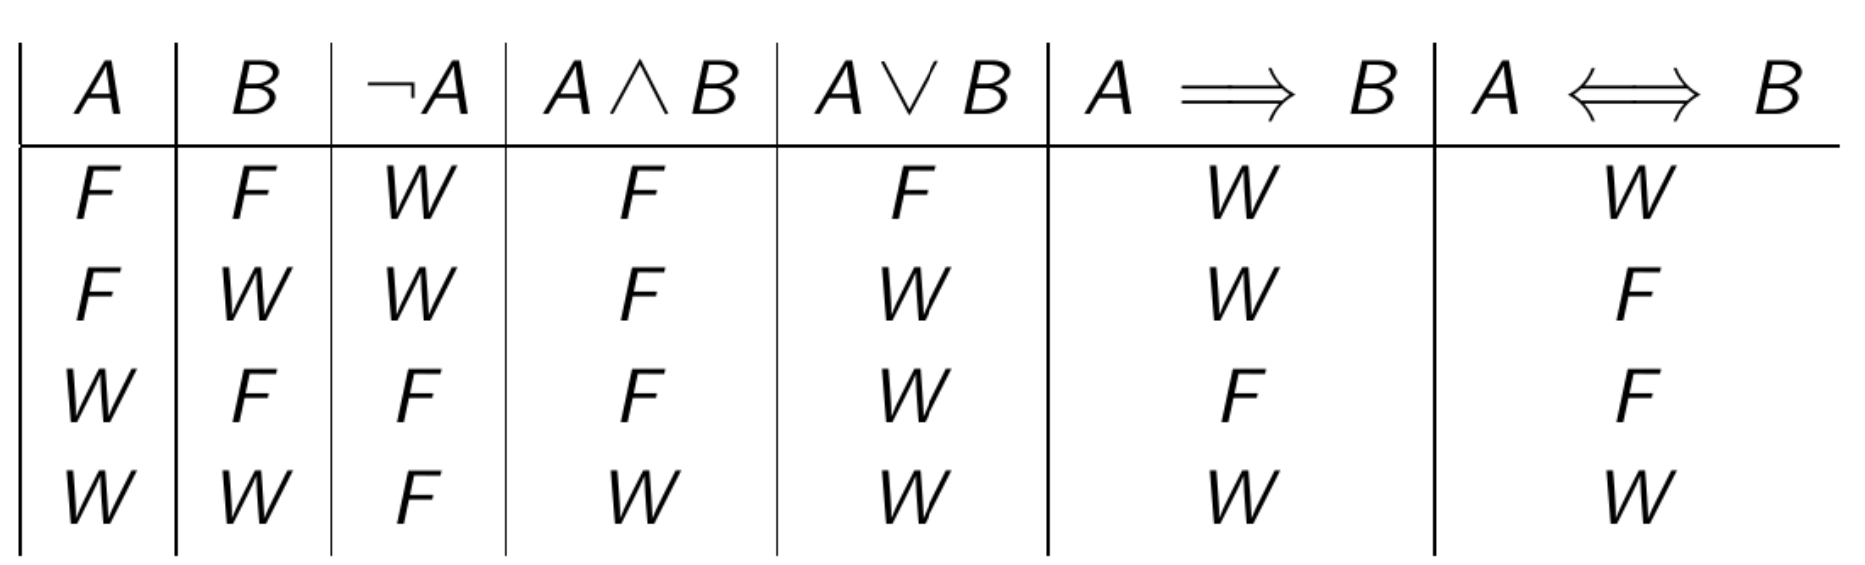
\includegraphics[width = 8 cm]{Wahrheitstafel.png}
\end{center}
\end{remark}
\subsection[]{Beweise}
\begin{definition}
Direkter Beweis:
\begin{center}
     Voraussetzung(en) $\Rightarrow$ Behauptung
\end{center}
\end{definition}
\begin{definition}
Indirekter Beweis:
\begin{center}
    $(A(x) \Rightarrow B(x)) \Leftrightarrow (\neg B(x) \Rightarrow \neg A(x))$
\end{center}
\end{definition}
\begin{definition}
Widerspruchsbeweis:\\
Wir möchten die Wahrheit der Aussage A beweisen.\\
Dafür:\\
1) wir nehmen an, dass $\neg$A gilt\\
2) wir finden einen Widerspruch (mit Annahmen, logischen Argumenten,...)\\
3) daraus folgt: A gilt.
\end{definition}
\begin{definition}
Das Prinzip der vollständigen Induktion:\\
Es sei eine Aussage $A$ zu beweisen, die von der natürlichen Zahl $n$ abhängt, $A(n)$.\\
Angenommen:\\
1) Die Aussage A(1) gilt (Induktionsanfang);\\
2) Für alle natürlichen Zahlen $m$:
\begin{center}
    falls $A(m)$ (Induktionsvoraussetzung) gilt, so gilt $A(m+1)$ (Induktionsschritt). 
\end{center}
Dann gilt $A(n)$ für alle natürlichen Zahlen.
\end{definition}
\subsection[]{Abbildungen, Kardinalität von Mengen und Relationen}
\begin{definition}
Seien $A,B$ Mengen. Eine Abbildung $\alpha$ von $A$ nach $B$ ist eine Relation des kartesischen Produkts $A \times B$, d.h $\alpha \subset A \times B$ mit der Eigenschaft
\begin{center}
    \textcolor{blue}{zu jedem Element $a \in A$ gibt es genau ein Element $b \in B$ derart, dass das Paar $(a,b)$ in $\alpha$ liegt. Es ist $b = \alpha(a)$.}
\end{center}
\end{definition}
\begin{definition}
Ist $a \in A$, so heißt $b=\alpha(a)$ das \textcolor{orange}{Bild von $a$} unter $\alpha$.
\end{definition}
\begin{definition}
Die Menge Bild$\alpha \coloneqq \{ b \in B : \exists a \in A : b = \alpha(a)\} = \{ \alpha(a) : a \in A\}$ heißt das \textcolor{orange}{Bild von $\alpha$}.
\end{definition}
\begin{definition}
Eine Abbildung $\alpha:A \rightarrow B$ heißt \textcolor{orange}{injektiv}, falls aus $\alpha(a) = \alpha(a')$ folgt stets $a = a'$.
\end{definition}
\begin{definition}
Eine Abbildung $\alpha:A \rightarrow B$ heißt \textcolor{orange}{surjektiv (auf B)}, falls Bild$\alpha = B$
\end{definition}
\begin{definition}
Eine Abbildung $\alpha:A \rightarrow B$ ist \textcolor{orange}{eine Bijektion von $A$ auf $B$}, falls $\alpha$ injektiv und surjektiv ist.
\end{definition}
\begin{definition}
Ist $N \subset B$, so definiert man die \textcolor{orange}{Urbildmenge} $\alpha^{-1}(N) \subset A$ durch 
\begin{center}
    $\alpha(N) =  \{a \in A : \alpha(a) \in N\}$
\end{center}
\end{definition}
\begin{definition}
Zwei Mengen $A,B$ heißen gleichmächtig ($A$ und $B$ haben die gleich Kardinalität) falls es eine Bijektion 
\begin{center}
    $f : A \rightarrow B$
\end{center}
gibt.
\end{definition}
\begin{definition}
\begin{enumerate}
    \item Die Menge $A$ heißt endlich, falls $A = \emptyset$, oder es gibt $n \in \mathbb{N}$, und eine Bijektion $f : \{1,2,...,n\} \rightarrow A$.
    \item In diesem Fall sagen wir, dass die Kardinalität von $A$, $n$ ist, und wir schreiben $\#(A) = |A| = n$.
\end{enumerate}
\end{definition}
\begin{definition}
Sei $A$ eine Menge mit $|A| = |\mathbb{N}|$, so heißt $A$ abzählbar unendlich.
\end{definition}
\begin{definition}
Eine Relation $R$ auf die Menge $M$ heißt
\begin{enumerate}
    \item \textcolor{red}{reflexiv}: falls $xRx$ gilt für jedes $x \in X$;
    \item \textcolor{red}{symmetrisch}: falls $xRy$ genau dann wenn $yRx$, für alle $x,y \in X$;
    \item \textcolor{red}{transitiv}: falls $xRz$ aus $xRy$ und $yRz$ folgt, für $x,y,z \in \mathbb{X}$.
\end{enumerate}
\end{definition}
\begin{definition}
Sei $X$ eine Menge, und ~ heißt \textcolor{orange}{Äquivalenzrelation} falls sie \textcolor{orange}{reflexiv}, \textcolor{orange}{symmetrisch} und \textcolor{orange}{transitiv} ist, d.h.
\begin{enumerate}
    \item für alle $x \in X$ gilt: $x \sim x$,
    \item für alle $x,y \in X$ gilt: $x \sim y \Leftrightarrow y \sim x$,
    \item für alle $x,y,z \in X$ gilt: aus $x \sim y$ und $y \sim z$ folgt $x \sim z$.
\end{enumerate}
\end{definition}
\begin{definition}
Sei $\sim$ eine Äquivalenzrelation auf die Menge $X$. Dann heißen, für $a \in X$, die Mengen
\begin{center}
$[a] \coloneqq \{x \in X : x \sim a\} =: [a]_\sim$
\end{center}
\textcolor{orange}{Äquivalenzklassen}(der Äquivalenzrelation $\sim$ ).
\end{definition}
\begin{definition}
Sei $X$ eine nicht leere Menge und $P \subset \mathcal{X}$. Dann heißt $P$ eine Partition falls:
\begin{enumerate}
    \item Für alle $A \in P$ gilt $A \neq \emptyset$,
    \item Für alle $A,B \in P$ gilt entweder $A=B$ oder $A \cap B = \emptyset$,
    \item Für alle $x \in X$ existiert $A \in P$ so, dass $x \in A$.
\end{enumerate}
\end{definition}
\begin{corollary}
Sei $X$ eine nicht leere Menge und $\sim$ eine Äquivalenzrelation auf $X$. Dann ist die Menge aller Äquivalenzklassen von $\sim$, nämlich $X/\sim$ eine Partition von $X$. 
\end{corollary}

\section{Algebraische Strukturen}
\begin{definition}
Ein Körper $\mathbb{K}$ $(K,+,\cdot,0,1)$ ist eine nicht leere Menge $K$ auf die eine
\begin{enumerate}
    \item \textbf{Addition}\\
    $+ :K\times K\rightarrow K$\\
    $(a,b) \mapsto a + b$
    \item und eine \textbf{Multiplikation (Produkt)}\\
    $\cdot :K\times K\rightarrow K$\\
    $(a,b) \mapsto a \cdot b$,
\end{enumerate}
definiert sind, so dass die Eigenschaften (A1), (A2), (A3), (A4), (M1), (M2), (M3), (M4) und (D) erfüllt sind.
\begin{itemize}
    \item \textcolor{blue}{(A1) Assoziativität:} Für alle $a,b,c \in K$ gilt
    \begin{center}
        $a + (b + c) = (a + b) + c$
    \end{center}
    \item \textcolor{blue}{(A2) Kommutativität:} Für alle $a,b \in K$ gilt
    \begin{center}
        $a + b = b + a$
    \end{center}
    \item \textcolor{blue}{(A3)} Es gibt ein Nullelement in $K$, \textcolor{blue}{das Nullelement}, welches wir mit 0 bezeichnen, mit der Eigenschaft, dass für alle $k \in K$
    \begin{center}
        $0 + k = k + 0 = k$
    \end{center}
    \item \textcolor{blue}{(A4)} Zu jedem $a \in K$ gibt es ein Element in $K$, welches wir mit $-a$ bezeichnen, mit
    \begin{center}
        $a + (-a) = (-a) + a = 0$,
    \end{center}
    Das Element $-a$ ist das \textcolor{blue}{zu a inverse Element bzgl. der Addition +}, oder das additive Inverse von $a$.
    \item \textcolor{blue}{(M1) Assoziativität:} Für alle $a,b,c \in K$ gilt
    \begin{center}
        $a \cdot (b \cdot c) = (a \cdot b) \cdot c$
    \end{center}
    \item \textcolor{blue}{(M2) Kommutativität:} Für alle $a,b \in K$ gilt
    \begin{center}
        $a \cdot b = b \cdot a$
    \end{center}
    \item \textcolor{blue}{(M3)} Es gibt ein Element in $K$, \textcolor{blue}{das Einzelelement}, welches wir mit 1 bezeichnen und verschieden von 0 ist, mit der Eigenschaft, für alle $k \in K$
    \begin{center}
        $1 \cdot k = k \cdot 1 = k$
    \end{center}
    \item \textcolor{blue}{(M4)} Zu jedem $a \in K\diagdown \{0\}$, gibt es ein Element in $K$ , welches wir mit $a^{-1}$ bezeichnen, mit
    \begin{center}
        $a \cdot a^{-1} = a^{-1} \cdot a = 1$,
    \end{center}
    Das Element $a^{-1}$ ist das \textcolor{blue}{zu a inverse Element bzgl. der Multiplikation $\cdot$}, oder das multiplikativ Inverse von a.
    \item \textcolor{blue}{(D) Distributivität} Für alle $a,b,c \in K$ gilt
    \begin{center}
        $(a + b) \cdot c = a \cdot c + b \cdot c$\\
        $a \cdot (b + c) = a \cdot b + a \cdot c$
    \end{center}
\end{itemize}
\end{definition}
\begin{definition}
\begin{itemize}
    \item \textcolor{blue}{(a)} Sei $\mathbb{K}$ ein Körper. Dann ist $(\mathbb{K} \diagdown \{0\}, \cdot, 1)$ \textcolor{red}{assoziativ}, hat ein \textcolor{blue}{neutrales Element}, 1, und jedes Element $k \in \mathbb{K} \diagdown \{0\}$ hat ein \textcolor{green}{multiplikatives Inverses}. Eine Menge mit einer Operation die diese drei Eigenschaften hat ist eine \textcolor{orange}{Gruppe}.
\end{itemize}
\end{definition}
\begin{definition}
Eine Gruppe ist ein Paar $(G, \ast)$, welches aus einer nicht leeren Menge $G$, und einer Operation
\begin{center}
    $\ast : G \times G \rightarrow G$\\
    $(g,h) \mapsto g \ast h$
\end{center}
besteht, welche die folgenden Eigenschaften erfüllt.
\begin{itemize}
    \item \textcolor{blue}{G1} $(g_1 \ast g_2) \ast g_3 = g_1 \ast (g_2 \ast g_3)$ für alle $g_1, g_2, g_3 \in G$
    \item \textcolor{blue}{G2} Es existiert ein Element $e \in G$ so, dass $e \ast g = g$ für alle $g \in G$
    \item \textcolor{blue}{G3} Für jedes $g \in G$ existiert $g' \in G$ so, dass $g' \ast g = e$.
\end{itemize}
Ein Element mit der Eigenschaft (G2) nennt man neutrales Element der der Gruppe. Für $g \in G$ nennt man ein Element mit der Eigenschaft (G3) Inverses zu $g$ und notiert es mit $g^{-1}$.
\end{definition}
\begin{definition}
Eine Menge $M$ mit zwei Operationen + und $\cdot$, so dass (A1), (A2), (A3), (A4) sind in Bezug auf $\cdot$ erfüllt, und die Eigenschaft (D) ist auch erfüllt, heißt ein \textcolor{orange}{Ring}. Wenn dazu noch (M3) erfüllt ist, so heißt es \textcolor{red}{Ring mit 1}.\\
Ein Ring mit 1, der (M2) und (M4) erfüllt ist ein Körper.
\end{definition}
\begin{proposition}
Das bzgl. + inverse Element 0 in einem Körper $\mathbb{K} = (K, *, \cdot, 0, 1)$ ist eindeutig. Weiterhin, gibt es außer 0 kein weiteres Element $a \in K$ so, dass $k + a= k$ für alle $k \in K$.\\
Das bzgl, $\cdot$ inverse Element 1 in einem Körper $\mathbb{K} = (K, *, \cdot, 0, 1)$ ist eindeutig. Weiterhin, gibt es außer 1 kein weiteres Element $a \in K$ so, dass $k \cdot a = k$ für alle $k \in K$.
\end{proposition}
\begin{theorem}
Sei $m \in \mathbb{N}$. Dann ist $(\mathbb{Z}_m, +, \cdot, [0], [1])$ ein kommutativer Ring mit 1, d.h. die Eigenschaften (A1), (A2), (A3), (A4), (M1), (M2), (M3) und (D) sind erfüllt.
\end{theorem}
\begin{theorem}
Sei $p \in \mathbb{N}$ eine Primzahl. Dann ist $(\mathbb{Z}_p, +, \cdot, [0], [1])$ ein Körper.
\end{theorem}
\begin{definition}
Sei $\mathbb{K}$ ein Körper.
\begin{center}
    $\mathbb{K}[x] \coloneqq \{\sum_{i = 0}^m a_ix^i : a_i \in \mathbb{K}, m \in \mathbb{N}\}$
\end{center}
ist die Menge aller Polynome über $\mathbb{K}$ (d.h., die Koeffizienten sind Elemente aus $\mathbb{K}$).\\
Mit den folgenden Operationen wird $\mathbb{K}[x]$ ein (Polynom-)Ring:
\begin{enumerate}
    \item $+ : \mathbb{K}[x] \times \mathbb{K}[x] \rightarrow \mathbb{K}[x]$\\
    $(\sum_{i=0}^m a_ix^i, \sum_{i=0}^n b_ix^i) \mapsto \sum_{i=0}^{max\{n,m\}} (a_i + b_i)x^i$\\
    wobei für $i > m ($bzw.$ j > n) a_i = 0$ (bzw. $b_j = 0)$ ist.
    \item $\cdot :\mathbb{K}[x] \times \mathbb{K}[x] \rightarrow \mathbb{K}[x]$\\
    $(\sum_{i=0}^m a_ix^i, \sum_{i=0}^n b_ix^i) \mapsto \sum_{i=0}^{m+n}(\sum_{k=0}^i a_kb_{i-k})x^i$\\
    Es folgt aus den Eigenschaften des Körpers $\mathbb{K}$ und der Definition von $\mathbb{K}[x]$, dass $(\mathbb{K}[x],+,\cdot)$ ein Ring mit $1 = 1_{\mathbb{K}}$ ist.
\end{enumerate}
\end{definition}
\begin{definition}
Eine Permutation der Zahlen $\{!, \dots, n\}$ ist eine bijektive Abbildung $\pi:\{1, \dots,n\} \rightarrow \{1, \dots, n\}$. Die Menge aller Permuationen von  $1, \dots,n$ wird mit \textcolor{orange}{$S_{n}$} bezeichnet, und bildet mit der Komposition von Abbildungen, eine Gruppe, und diese heißt \textcolor{orange}{symmetrische Gruppe} zum Index $n$. Weiterhin hat die Gruppe $n!$ Elemente.
\end{definition}
\begin{definition}
Sei $\pi \in S_n$ eine Permutation von $\{1,\dots,n\}$. Ein Fehlstand von $\pi$ ist ein Indexpaar $(i,j)$ mit $1 \leq i < j \leq n$ und $\pi(i) > \pi(j)$. Es ist 
\begin{center}
    \textcolor{blue}{Fehl($\pi$) = $\{(i,j) : (i,j)$ ein Fehlstand von $\pi \}$}      und\\
    \textcolor{cyan}{sgn($\pi) = (-1)^{Fehl(\pi)}$}
\end{center}
\end{definition}

\section{Vektorräume}
\begin{definition}
    Sei $\K$ ein Körper. Ein Vektorraum $V=(V,+,\cdot)$ über $\K$ ist eine Menge $V$ für die
    \begin{itemize}
        \item Eine Summe (Addition)
            \begin{align*}
                +:&V \times V \to V \\
                &(x,y) \mapsto x+y
            \end{align*}
        \item Ein Produkt (Skalarmultiplikation/ Produkt mit Skalaren)
            \begin{align*}
                \cdot :&\K\times V \to V \\
                &(\lambda ,y) \mapsto \lambda \cdot y
            \end{align*}
    \end{itemize}
    gegeben sind, so dass die folgenden Eigenschaften erfüllt sind:\\
    \begin{itemize}[]
        \item (A1) $(x+y)+z=x+(y+z)$ für alle $x,y,z\in V$,
        \item (A2) $x+y=y+x$ für alle $x,y\in V$,
        \item (A3) Es existiert ein Element in $V$, der Nullvektor, welchen wir mit $0=0_V$ bezeichnen, für den gilt $0_V+x=x+0_V=x$ für alle $x\in V$,
        \item (A4) Für jedes $x\in V$ gibt es genau ein Element in $V$, welches mit $-x$ bezeichnet wird, für das gilt $x+(-x)=(-x)+x=0_V$
    \end{itemize}
    und
    \begin{itemize}
        \item (P1) $(a\cdot b)\cdot x=a\cdot (b\cdot x)$ für $a,b\in \K,x\in V$,
        \item (P2) $1_\K\cdot x = x$ für alle $x\in V$,
        \item (P3) $a\cdot(x+y) = a\cdot x +a\cdot y$ für alle $a\in \K,x,y\in V$,
        \item (P4) $(a+b)\cdot x = a\cdot x + b\cdot x$ für alle $a,b\in \K, x\in V$.
    \end{itemize}
\end{definition}

\begin{remark}
    Sei $V=(V,+,\cdot)$ ein VR über den Körper $\K$
    \begin{enumerate}
        \item $(V,+,0_V)$ ist eine Gruppe, da (A1),(A3),(A4) erfüllt sind. Es gilt auch (A2), und somit ist + kommitativ.
        \item Eine Gruppe $(G,\circ,e)$, die (A2) erfüllt heißt abelsch (oder kommutativ) (Hier bezeichnet e das neutrale Element von Gin Bezug auf $\circ$
    \end{enumerate}
\end{remark}
\newpage
\begin{lemma}
 In einem $\K$-VR $V$ gilt für alle $v\in V$ und $\lambda \in \K$:
 \begin{enumerate}
    \item $0_\K \cdot v = 0_V$ und $\lambda \cdot 0_v = 0_V$
    \item $(-\lambda)\cdot v = -\lambda \cdot v=\lambda(-v)$. Insbesondere $(-1)\cdot v = -v$.
    \item $\lambda \cdot v = 0 \leftrightarrow \lambda = 0_\K$ oder $v=0_v$ (in $V$)
 \end{enumerate}
\end{lemma}

\begin{definition}
    Sei $\K$ ein Körper und $V$ ein $\K$-VR.
    \begin{enumerate}
        \item Sei $m\in\N_0$ und $v_1,\dotsb,v_m \in V$. Dann ist $w\in V $ eine Linearkombination von $v_1\dotsb,v_m$ falls $\lambda_1,\dotsb,\lambda_m\in \K$ esistieren mit (ist $m=0$, so haben wir Keinen Vektor)
        \begin{align*}
            w=\lambda_1 \cdot v_1+\dotsb \lambda_m\cdot v_m
        \end{align*}
        \item Sei $S\subset V$ und $w\in V$. Der Vektor $w\in V$ ist eine Linearkombination von Vektoren aus $S$ falls es $m \in \N_0, \lambda_1,\dotsb,v_m\in\K,v_1,\dotsb,v_m\in S$ gibt, mit
        \begin{align*}
            w=\lambda_1 \cdot v_1 + \dotsb + \lambda_m v_m = \sum_{i=1}^{m}\lambda_1\cdot v_i
        \end{align*}
    \end{enumerate}
\end{definition}

\begin{definition}
    Sei $\K$ ein Körper und $V$ ein $\K$-VR. Die Teilmenge $U\subset V$ heißt Unterraum (oder Untervektorraum, oder linearer Teilraum) von $V $, wenn $(U,+,\cdot) $ ein Vektorraum ist, wobei $+$ und $\cdot$ die im Vektorraum $V=(V,+,\cdot)$ definierten Operationen sind.\\
    Eigene(Lennarts zugabe): Der Unterraum eines Vektorraums ist auch ein Vektorraum\\
    \\
    Unterraumkriterium:\\
    Sei $\K$ ein Körper und $V$ ein $\K$-VR. Die Teilmenge $U\subset V $ ist ein Unterraum von $V$ genau dann, wenn
    \begin{enumerate}
        \item (U1) $U\neq \emptyset$
        \item (U2) für alle $x,y\in U$ ist $x+y\in U$
        \item (U3) für alle $\lambda \in \K$ und $x\in U$ ist $\lambda\cdot x \in U$
    \end{enumerate}
\end{definition}
\newpage
\begin{remark}
\quad \\
    \begin{enumerate}
        \item ist $(V,+,\cdot)$ ein VR und $U$ ein Unterraum von $V$, so  ist $0_V=0_U$.
        \item Dotation: Wir schreiben $U\leq V$um zu bezeichnen, dass $U$ ein Unterraum von $V$ ist,d.h.,
        \begin{enumerate}
            \item $U\subset V$
            \item $U$ hat die Vektorraumstruktur mit den von $V$ vererbten Operationen $+,\cdot$
        \end{enumerate}
    \end{enumerate}
\end{remark}

\begin{proposition}
Sei $V $ein $\K$-VR. Sind $W_i, i\in I$, Unterräume von V, so ist 
\begin{align*}
    \bigcap_{i\in I} W_i \leq V
\end{align*}
auch ein Unterraum von V.
\end{proposition}

\begin{definition}
    Sei $V$ ein $\K$-VR und $M\subset V$ eine Teilmenge von $V$. Dann heißt
    \begin{align*}
        \text{lin} M&\coloneqq \bigcap\{U\ :\ M\subset U,\ U\leq V\text{ ist ein Unterraum von } V\} \\
        &= \bigcap_{M\subset U\leq V}U
    \end{align*}
    von $M$ erzeugter Unterraum, von $M$ aufgespannter Unterraum, Erzeugnis oder lineare hülle von $M$.
    \begin{itemize}
        \item Alternative Notation für die lineare Hülle: span$M$ oder $\langle M\rangle$
        \item Aus Proposition (die vorherige) folgt, dass lin$M$ ein Unterraum von $V$ ist, da der Durchschnitt nicht leer ist: $M\subset V$ und $ V\leq V$
        \item lin$\emptyset = \{0\}$
    \end{itemize}
\end{definition}

\begin{theorem}
Sei $V$ ein $\K$-VR und $M\subset V$ eine nicht leere Teilmenge.
Dann besteht lin$M$ aus allen Linearkombinationen von $M$ d.h.,
\begin{align*}
    \text{lin} M =\left\{\sum_{i=0}^n \alpha_i v_i\ :\ n\in\N,\alpha_i\in\K,v_i \in M,\ 1\leq i\leq n\right\}
\end{align*}
\end{theorem}

\begin{definition}
    Sei $\mathcal{M}$ eine Menge von Unterräumen von $V$. Die Summe dieser Menge $\mathcal{M}$ ist
    \begin{align*}
        \sum \mathcal{M} = \sum_{U\in \mathcal{M}} \coloneqq \left\{ u_1+\dotsb + u_n\ :\ \N_0, u_i\in\bigcup \mathcal{M} \text{ für } 1\leq i \leq n \right\}
    \end{align*}
    \begin{itemize}
        \item Für endlich viele $U_1,\dotsb, U_m\leq V$ ist 
        \begin{align*}
            U_1+\dotsb+U_m=\{u_1+\dotsb+u_m \ :\ u_i \in U_i, 1\leq i \leq m\}
        \end{align*}
        \item Ist $\mathcal{M}=\emptyset$, so ist $\sum \mathcal{M}=\{0_V\}$
    \end{itemize}
\end{definition}

\begin{theorem}
Sei $\mathcal{M}$ eine Menge von Unterräumen von $V$. Die Summe $\sum\mathcal{M}$ ist ein Unterraum von $V$.
\end{theorem}

\begin{definition}
$0_V$ lässt sich \textit{nicht-trivial} als Linearkombination von $v_1,\dotsb,v_m\in V$ darstellen, $m\in \N_0$, d
falls es $\alpha_i\in\K, i=1,\dotsb m$ gibt, mit 
\begin{itemize}
    \item $\alpha_1v_1+\dotsb\alpha_m v_m = 0_V$
    \item mindestens ein $\alpha_i, i=1,\dotsb,m$, ist nicht Null (in $\K$).
\end{itemize}
\end{definition}

\begin{remark}
Die Vektoren $v_1,\dotsb,v_m$ in der vorigen Definition müssen nicht notwendigerweise paarweise verschieden sein!
\begin{align*}
    0=v_1+(-1)v_1
\end{align*}
mit $v_1\neq0_V$ und so ist $0_V$ eine \textit{nicht-triviale Linearkombination} von $v_1,v_2\coloneqq-v_1$.
\end{remark}

\begin{definition}
Sei $M\subset V$. Dann ist $M$ linear abhängig falls es $m\in \N$ und $v_1,\dotsb,v_m\in V$ paarweise verschieden gibt, so dass sich $0_V$ als \textit{nicht-triviale Linearkombination}
von $v_1,\dotsb,v_m$ darstellen lässt.\\
Ist $M$ nicht linear abhängig, so ist $M$ linear unabhängig.
\end{definition}

\begin{theorem}
Sei $V$ ein $\K$-VR und $M\subset V$. Genau dann ist M linear unabhängig, wenn aus
\begin{align*}
    0=\alpha_1 v_1 +\dotsb+\alpha_m v_m
\end{align*}
für $m\in\N_0$ und $v_1,\dotsb,v_m\in M$ paarweise verschieden und $\alpha_1,\dotsb,\alpha_m\in\K$, folgt, dass $\alpha_1=\dotsb=\alpha_m=0$.
\end{theorem}

\begin{theorem}
Sei $V$ ein $\K$-VR und $M\subset V$.
\begin{itemize}
    \item Genau dann ist $M$ linear abhängig, wenn $v\in M$ existiert mit 
    \begin{align*}
        \text{lin}(M\backslash\{v\})=\text{lin}M.
    \end{align*}
    \item Genau dann ist $M$ linear unabhängig, wenn für alle $v\in M$ gilt
    \begin{align*}
        \text{lin}(M\backslash\{v\})\neq\text{lin}M.
    \end{align*}
\end{itemize}
\end{theorem}

\begin{remark}
Sei$V$ ein $\K$-VR und seien $M_1\subset M_2 \subset V$.
\begin{itemize}
    \item Ist $M_1$ l.a., so ist auch $M_2$ linear abhängig.
    \item Ist $M_2$ l.u., so ist auch $M_1$ linear unabhängig.
\end{itemize}
\end{remark}

\begin{definition}
Sei $V$ ein $\K$-VR und $B\subset V$ eine Teilmenge. Die Teilmenge $B$ ist eine Basis von $V$ wenn:
\begin{enumerate}
    \item  $V=$lin$B$, d.h., $V$ ist das Erzeugnis von $B$ (oder $B$ ist das Erzeugendensystem von V)
    \item $B$ ist l.u.
\end{enumerate}
Für den Nullraum$\{0_V\}=$lin$\emptyset$, definieren wir $\emptyset$ als Basis
\end{definition}

\begin{remark}
Ist $B = \{v_1,\dotsb, v_m\}$ eine endliche Basis von $V$, mit paarweise verschiedenen Elementen $v_1,\dotsb, v_m$, so sagen wir auch $\text{“}v_1,\dotsb, v_m$ bilden eine Basis von $V\text{”}$.
\end{remark}

\begin{definition}
Ist $V$ ein $\K$-VR und ist $\{v_1,\dotsb, v_n\}$ eine Basis von $V$, mit paarweise verschiedenen Elementen, so nennen wir $(v_1,\dotsb, v_n)$ eine geordnete Basis von $V$
\end{definition}

\begin{theorem}
Sei $V$ ein $\K$-VR und $M\subset V$. Genau dann ist $M$ l.u., wenn jedes $v \in $lin$ M $ sich auf genau eine Weise als Linearkombination von paarweise verschiedenen Vektoren aus $M$ darstellen lässt.
\end{theorem}

\begin{theorem}
Seien $v_1,\dotsb,v_m\in V, 1\leq i\leq m$. Genau dann ist $\{v_1,\dotsb,v_m\}$ eine Basis des $\K$-VR $V$, falls für alle $v\in V$ gilt:
\begin{item}
$v=\sum_{i=1}^m k_i v_i$ mit geeigneten $k_i\in\K, 1\leq i \leq m$
\item Ist $v=\sum_{i=1}^m k_i v_i=\sum_{i=1}^m k_i' v_i$ so ist $k_i=k_i', 1\leq i \leq m$
\end{item}
Mit anderen Wörtern: Genau dann ist $\{v_1,\dotsb,v_m\}$ eine Basis von $V$, wenn jedes $v\in V$ eine eindeutige Linearkombination der $v_i$ ist.
\end{theorem}

\newpage
\section{Lineare (Un-)Abhängigkeit und Basen}
\input{Topics/4_Lineare_Un-_Abhängigkeit_Basen}
\section{Dimension \& co}
\Mundus
\section{Lineare Abbildungen}
\begin{definition}
Seien $V,\ W$ $\K$-Vektorräume und $T:V\to W$ eine Abbildung.
Dann heißt $T$ linear (auch $\K$ linear um den Körper zu betonen)(und auch Vektorraum \textit{Homomorphismus}), wenn
\begin{itemize}
    \item Für alle $v_1,\ v_2\in V$ gilt $T(v_1+v_2)=T(v_1)+T(v_2)$
    \item Für alle $\lambda\in\K$ und $v \in V$ gilt $T(\lambda\cdot v)=\lambda\cdot T(v)$
    \item $T(\lambda_1 v_1+\lambda_2 v_2)=\lambda_1T(v_1)+\lambda_2T(v_2)$
\end{itemize}
\end{definition}

\begin{proposition}
Sei $\K$ ein Körper und sei $T:V \to W$ eine lineare Abbildung.
Dann ist 
\begin{enumerate}
    \item $T(0_V)=0_W$
    \item Für $v_1,\dotsb,v_m \in V$ und $\lambda_1,\dotsb,\lambda_m$ gilt
    \begin{align*}
        T\left(\sum_{i=1}^m\lambda_iv_i\right)=\sum_{i=1}^m\lambda_iT(v_i)
    \end{align*}
\end{enumerate}
\end{proposition}

\begin{lemma}
Sei $\K$ ein Körper und seien $V,W$ und $W'$ Vektorräume über $\K$.
\begin{enumerate}[1.]
    \item Ist $T:V\to W$ linear, und $\alpha\in\K$, so ist 
    \begin{align*}
        (\alpha\cdot T):&V\to W\\
        &v \mapsto (\alpha\cdot T)(v)\coloneqq \alpha\cdot T(v) \text{   mit } \alpha T(v)\in W
    \end{align*}
    auch eine lineare Abbildung
    \item Sind $T_1,T_2:V\to W$ lineare Abbildungen, so ist 
    \begin{align*}
        (T_1+T_2):&V\to W\\
        &v \mapsto (T_1+T_2)(v)\coloneqq T_1(v)+T_2(v) \text{   mit } T_1(v)+T_2(v)\in W
    \end{align*}
    auch eine lineare Abbildung
    \item Sind $T_1:V\to W$ und $T_2:W\to W'$ lineare Abbildungen, so ist die Abbildung
    \begin{align*}
        (T_2\circ T_1):&V\to W'\\
        &v\mapsto (T_2\circ T_1)(v)=(T_2(T_1(v)))
    \end{align*}
    auch linear.
\end{enumerate}
\end{lemma}

\begin{theorem}
Sei $V$ ein endlich dimensionaler Vektorraum über $\K$, und sei $B=(b_1,\dotsb,b_n)$ eine geordnete Basis von $V$. Seien $w_1,\dotsb,w_n\in W$ beliebige Vektoren aus $W$.\\
Es existiert gena eine lineare Abbildung $T:V\to W$ so, dass $T(b_i)=w_i$ für $1\leq i\leq n$. Explizit ist $T$ wie folgt angegeben: ist $v\in V$, mit $v=\sum_{i=1}^n\lambda_i b_i$. Dann ist 
\begin{align*}
    T(v)=T\left(\sum_{i=1}^n\lambda_i b_i\right) = \sum_{i=1}^n\lambda_i w_i
\end{align*}
\end{theorem}

\begin{definition}\,
\textcolor{red}{Kern und Bild}\\
Seien $V,W$ Vektorräume über den Körper $\K$ und $T:V\to W$ eine lineare Abbildung.
\begin{enumerate}[1.]
    \item Der \textit{Kern} von $T$ ist
    \begin{align*}
        \text{Kern}(T)=\{v\in V, T(v)=0_W\} \quad (=\text{Kern}T)
    \end{align*}
    \item Das \textit{Bild} von $T$ ist 
    \begin{align*}
        \text{Bild}(T)&=\{w\in W:\exists v\in V \text{ mit } T(v)=w\}\\
        &=\{T(v):v\in V\} \quad (=\text{Bild}T)
    \end{align*}
\end{enumerate}
\end{definition}

\begin{theorem}
Seien $V,W$ VR über den Körper $\K$ und $T:V\to W$ eine lineare Abbildung. Dann ist 
\begin{enumerate}
    \item Kern$(T)\leq V$ ein Unterraum von $V$
    \item Bild$(T)\leq W$ ein Unterraum von $W$
\end{enumerate}
\end{theorem}

\begin{definition}
Seien $V,W$ VR über den Körper $\K$, $V$ endlich dimensional und $T:V\to W$ eine lineare Abbildung. Dann nennen wir Rang($T$)=$\text{dim}_\K$(Bild$T$) den Rang von $T$.
\end{definition}

\begin{remark}
Seien $V,W$ VR über den Körper $\K$. Sei $E\subset V$ ein Erzeugendensystem von $V$ und $T:V\to W$ eine lineare Abbildung. Es gilt Bild$T=$lin$\{ T(e):e\in E\}$.
Insbesondere, ist $E=\{v_1,\dotsb,v_m\}$, so ist 
\begin{align*}
    \text{Bild}T=\text{lin}\{T(v_1),\dotsb,T(v_m)\}
\end{align*}
\end{remark}

\begin{corollary}
Seien $V,W$ VR über den Körper $\K$. Sei $E=\{v_1,\dotsb,v_m\}\subset V$ ein Erzeugendensystem von $V$ und $T:V\to W$ eine lineare Abbildung. Es gilt 
\begin{align*}
    \text{Rang}T=\text{Rang}(T(v_1),\dotsb,T(v_m)).
\end{align*}
\end{corollary}

\begin{proposition}
\textcolor{red}{Injektivität und Surjektivität}\\
Seien $V,W$ VR über den Körper $\K$ und sei $T:V\to W$ eine lineare Abbildung.
\begin{enumerate}[1.]
    \item $T$ ist genau dann \textit{injektiv}, wenn Kern$T=\{0\}$.
    \item Seien $V,W$ endlich dimensionale Vektorräume. $T$ ist genau dann \textit{surjektiv}, wenn Rang$T=\text{dim}_\K W$.
\end{enumerate}
\end{proposition}

\begin{theorem}
\textcolor{red}{Dimensionssatz}\\
Seien $V,W$ endlich dimensionale Vektorräume über den Körper $\K$ und sei $T:V\to W$ eine lineare Abbildung. Es gilt
\begin{align*}
    \text{dimKern}T+\text{dimBild}T=\text{dim}V
\end{align*}
\end{theorem}
\section{Von Matrizen zu linearen Abbildungen und zurück}
Thema fängt in der letzten Vorlesung vom vorherigen Kapitel an.
\section{Etwas multilineare Algebra. Die Determinante}
\newcommand{\vol}[1]{\ensuremath{\txt{vol}\left(#1\right)}}
\begin{definition}[Determinante $1\times 1$ und $2\times 2$ Matrizen]
    \begin{itemize}
        \item Für $a \in \calM_1 (\mathbb{K})$ gilt $\det a = a$.
        \item Sei $a \coloneqq \matrx{a&b\\c&d}$ Es ist $\det a = ad-bc$. 
    \end{itemize}
\end{definition}
\begin{definition}[Laplace Entwicklung]
    Ist $n\geq 2$ und $A\in \calM_(\K)$, so ist \[
        \det A = \sum_{j=1}^n (-1)^{1+j} a_{1j}\det A_{1j}\]    
\end{definition}
\begin{definition}[Sarrus-Regel]
    Für $A\in \calM_3$ gilt \[
        \det A = a_{11}a_{22}a_{33} - a_{12}a_{21}a_{33} - a_{13}a_{22}a_{31} + 
        a_{12}a_{23}a_{31} + a_{13}a_{21}a_{32} - a_{11}a_{23}a_{32}\]
\end{definition}
\begin{definition}[Determinantenabbildung]
    Eine Determinantenabbildung auf $\calMn(\K)$ ist eine Abbildung $D:\calMn(\K)
    \to \K$ so, dass\begin{enumerate}
        \item $\forall i \in \set{1,\dots, n}$ ist $D$ linear in der i-ten Zeile,
        also \[
            D\left(\matrx{a_1\\\vdots\\a_i+\lambda b_i\\\vdots\\v_n}\right) = 
            D\left(\matrx{a_1\\\vdots\\a_i\\\vdots\\a_n}\right) + \lambda D\left(\matrx{
                a_1\\\vdots\\b_i\\\vdots\\a_n
            }\right)\]
        \item Hat $A\in \calMn(\K)$ zwei gleiche Zahlen, so ist $D(A) = 0$ (d.h.
        $D$ ist alternierend) 
        \item $D(I_n) = 1$
    \end{enumerate}    
\end{definition}
\begin{theorem}\hfill\break
    \begin{enumerate}[(i)]
        \item \[
            \det A = \sum_{j=1}^n (-1)^{1+j}a_{1j}\det A_{1j}\]
        \item \[
            \det A = \sum_{\sigma\in S_n}\txt{sgn}(\sigma)\prod_{i=1}^n a_{1\sigma}(i)\]
            mit $S_n :$ Permutationen von $\set{1,2,\dots,n}$ und sgn$(\sigma):$ 
            Fehltstände oder Signum von $\sigma$
        \item \[\abs{\det\matrx{a&b\\c&d}} = \abs{ad-bc}\equiv\txt{Fläche des 
        von $\matrx{a\\c}, \matrx{b\\c}$ aufgespannten Parallelogram.}\]
        \item Determinantenabbildung $
            D:\calMn(\K) \to \K:$\begin{enumerate}
                \item Linear in jeder Zeile
                \item Hat die Matrix $A\in \calMn(\K)$ zwei gleiche Zeilen, so ist 
                $\det A = 0$
                \item $\det I_n = n$
            \end{enumerate}
    \end{enumerate}
\end{theorem}
\begin{remark}
    Man sucht in der Definition der Determinante die \glqq Eigenschaften des Volumens\grqq
    in jeder Dimension, z.B. vol$(\lambda K) = \lambda^2$vol$(K), K\subset\R^2$.
    \newline\textbf{Geometrische Motivation} \begin{enumerate}
        \item Volumen ist Null wenn die 3 Vektoren auf einer Ebene liegen
        \item Volumen des Wuerfels mit Kantenlänge 1 ist 1 
        \item Verdoppelt man $v_1,v_2,v_3$ so wird das Volumen 8 mal größer \[
            \vol{\lambda_1v_1, \lambda_2v_2, \lambda_3v_3} = \lambda_1\lambda_2
            \lambda_3\vol{v_1,v_2,v_3}\]
    \end{enumerate}
    Volumen von Vektoren ist als Volumen des von $v_1,v_2,v_3$ aufgespannten 
    Parallelepiped zu verstehen. Vektoren in einer Determinante sind in Zeilen zu 
    verstehen.
    \newline\textbf{Die Determinante erfüllt:}\begin{enumerate}
        \item Determinante ist Null, wenn die 3 Vektoren l.a. sind
        \item Die Determinante der Einheitsmatrix ist 1
        \item $\det \matrx{\lambda_1x_1\\\lambda_2x_2\\\lambda_3x_3} = \lambda_1
        \lambda_2\lambda_3 \det\matrx{x_1\\x_2\\x_3}$
    \end{enumerate}
    Die Determinante erfüllt also all die Eigenschaften die wir geometrisch haben
    wollen.
\end{remark}
\begin{definition}
Sei $A \in \calMn(\mathbb{K})$. TFAE
\begin{enumerate}
    \item det $A \neq 0$
    \item $A$ ist invertierbar
    \item Es gibt $B \in \calMn(\mathbb{K})$ mit $AB = I_n$
    \item Rang$A=n$
    \item $T_A: \mathbb{K}^n \to \mathbb{K}^n, \quad x\mapsto Ax$ ist bijektiv
    \item $T_A: \mathbb{K}^n \to \mathbb{K}^n, \quad x\mapsto Ax$ ist surjektiv
    \item $T_A: \mathbb{K}^n \to \mathbb{K}^n, \quad x\mapsto Ax$ ist injetiv
    \item Kern$T_A=0$
    \item Es gibt Elementarmatrizen $R_1,...,R_k$ so, dass $A=R_k...R_1\cdot I_n$
    \item Mittels elementarer Zeilenumformungen bekommt man aus $A$ die Matrix $I_n$
    \end{enumerate}
\end{definition}

\begin{theorem}
Sei $D:\calMn(\mathbb{K}) \to \mathbb{K}$ eine Determinantenabbildung und sei \\ $A \in \calMn(\mathbb{K})$. Dann ist $A$ invertierbar genau dann, wenn $D(A) \neq 0$
\end{theorem}

\begin{theorem}
Falls eine Determinantenfunktion det$:\calMn(\mathbb{K}) \to \mathbb{K}$ existiert, so ist diese eindeutug bestimme. Also, es gibt höchstens eine Determinantenabbildung.
\end{theorem}

\begin{theorem}
Es gibt genau eine Determinantenabbildung auf $\mathbb{K}$ , nämlich
\begin{align*}
    \det A=\sum_{\sigma\in S_n}sgn(\sigma) \prod_{i=1}^n a_{i\sigma(i)}.
\end{align*}
Es reicht zu zeigen, dass det eine Determinantenabbildung ist, nach Satz (2 vorher)
\end{theorem}

\begin{theorem}
Sei $A\in \calMn(\mathbb{K})$. Dann gilt 
\begin{align*}
    \det A=\det A^T
\end{align*}
\end{theorem}

\begin{theorem}
Seien $A,B\in \calMn(\mathbb{K})$. Es gilt
\begin{align*}
    \det(AB)=\det A \det B.
\end{align*}
\end{theorem}

\begin{theorem}
Die menge der invertierbaren Matzizen
\begin{align*}
    GL(n,\mathbb{K}) \coloneqq \{A\in \calMn(\mathbb{K}) : \det A \neq 0\}
\end{align*}
ist eine Gruppe bzgl. der Matrixmultiplikation
\end{theorem}

\begin{theorem}
Sei $n\geq 2$ und $A=(a_{ij}) \in \calMn(\mathbb{K})$. Es gilt:
\begin{enumerate}
    \item Entwicklung nach der $i-$ten Zeile
    \begin{align*}
        \det A = \sum_{j=1}^n (-1)^{\textcolor{red}{i}+j}a_{\textcolor{red}{i}}\det A_{\textcolor{red}{i}j}
    \end{align*}
    \item Entwicklung nach der $j-$ten Spalte
    \begin{align*}
        \det A = \sum_{j=1}^n (-1)^{i+\textcolor{red}{j}}a_{i\textcolor{red}{j}}\det A_{i\textcolor{red}{j}}
    \end{align*}
\end{enumerate}
\end{theorem}
\section{Linearformen und Bilinearformen}
\begin{definition}
    Sei $f: V\to \K$ eine lineare Abbildung auf $V$. Dann heißt $f$ Linearform.
\end{definition}
\begin{definition}
    Die Menge aller linearen Abbildungen $f:V\to\K$ auf $V$ heißt Dualraum von V
    und wird mit $V^*$ notiert. Der Dualraum $V^*$ von $V$ ist mit den folgenden
    Operationen ein Vektorraum: $f,g \in V^*, \lambda \in \K,$ und $v\in V$
    \begin{align*}
        (f+g)(v) &\coloneqq f(v) + g(v)\\
        (\lambda f)(v) &\coloneqq \lambda(f(v))
    \end{align*}
\end{definition}
\begin{theorem}
    Sei $V$ ein endlich dimensionaler Vektorraum über einen Körper $\K$. Es ist
    \[
        \dim V = \dim V^*
    \]
\end{theorem}
\begin{proof}
    Später
\end{proof}
\begin{definition}
    Sei $V$ ein endlich dimensionaler Vektorraum über einen Körper $\K$, und $B
    = (v_1, \dots, v_n)$ eine Basis von $V$. Dann bezeichnen wir mit $v_i^* \in
    V^*$ die Linearform \[
        v_i^*\left(\dsum_{j=1}^n \lambda_i v_j\right) = \lambda_i, \midspace
         \lambda_i \in \K, 1\leq i \leq n\]
    und $(v_1^*, \dots, v_n^*)$ heißt duale Basis zu $B$.
\end{definition}


\section{Euklidische und unitäre Vektorräume \& etwas analytische Geometrie}
\newcommand{\stdscp}{\ensuremath{\scp{\cdot,\cdot}}}
\newcommand{\fuer}{\ensuremath{\text{ für }}}
\newcommand{\KeRoC}{(\K = \R \smallspace \lor \smallspace\K = \C)}
\begin{definition}
    Sei $V$ ein $\R$ Vektorraum. Eine positiv definite symmetrische Bilinearform
    auf $V$ heißt (euklidisches) Skalarprodukt. Ist $\stdscp$ ein 
    (euklidisches) Skalarprodukt auf den reellen Vektorraum $V$, so heißt $(V, 
    \stdscp)$ ein Euklidischer Vektorraum.
\end{definition}
\begin{example}
    Auf $\R^n$ ist $\scp{x,y} = x^T y$ ein euklidisches Skalarprodukt. Wir 
    nennen es Standard Skalarprodukt und es ist das Standardbeispiel eines 
    euklidischen (endlich-dimensionalen) Vektorraum.
\end{example}
\begin{definition}
    Sei $V$ ein komplexer Vektorraum und sei $\stdscp: V\times V\to
    \C$ eine Abbildung mit den folgenden Eigenschaften:\begin{enumerate}
        \item $\stdscp$ ist linear in der ersten Variable, d.h. \[
            \forall v_1, v_1', v_2 \in V \smallspace\forall \lambda \in \C: 
            \scp{\lambda v_1 + v_1', v_2} = \lambda\scp{v_1, v_2} + \scp{v_1',
             v_2}\]
        \item $\stdscp$ ist sesquilinear in der zweiten Variable, d.h
            \[
                \forall v_1, v_2, v_2' \in V \smallspace \forall \lambda \in \C
                : \smallspace \scp{v_1, \lambda v_2 + v_2'} = \compconj{\lambda}
                \scp{v_1, v_2} + \scp{v_1, v_2'}\]
    \end{enumerate}
    Dann heißt $\stdscp$ eine Sesquilinearform.
\end{definition}
\begin{definition}
    Eine Sesquilinearform auf den komplexen Vektorraum $V$ heißt\begin{itemize}
        \item hermitesch wenn zusätzlich gilt\[
            \scp{v_1, v_2} = \compconj{\scp{v_1,v_2}}\]
        \item positiv definit wenn \[
            \forall 0 \neq v \in V: \smallspace \scp{v,v} > 0\]
    \end{itemize}
\end{definition}
\begin{definition}
    Sei $V$ ein $\C$-Vektorraum. Eine positiv definite hermitesche 
    Sesquilinearform $\stdscp:V\times V\to \C$ auf $V$ heißt unitäres
    Skalarprodukt oder inneres Produkt. Ist $\stdscp$ ein inneres Produkt auf 
    den komplexen Vektorraum $V$, so heißt $(V, \stdscp)$ ein unitärer 
    Vektorraum.
\end{definition}
\begin{definition}
    Sei $(a_{ij}) = A\in \calM_{n\times m}(\C)$. Dann ist $A^H = (\compconj{
        a_{ij}})^T$ die hermitesch Transponierte von $A$. Sind alle Einträge von
        $A \in \calM_{n\times m}(\C)$ reell, so ist $A^H = A^T$.
\end{definition}
\begin{example}
    Auf $\C^n$ ist $\scp{x,y}= y^H x= \dsum_{i=1}^n \compconj{y_i}x_i$ ein 
    inneres Produkt. Wir nennen es Standard inneres Produkt und es ist das 
    Standardbeispiel eines unitären (endlich-dimensionalen) Vektorraums.
\end{example}
\begin{remark}
    \hfill
    \begin{enumerate}
        \item Ist $\stdscp$ ein inneres Produkt ($\K = \C$) oder ein 
        Skalarprodukt ($\K = \R$), so ist $\forall v \in V: \scp{v,v} \geq 0$ 
        \item Ein Unterraum eines euklidischen oder unitären Vektorraums ist 
        wieder ein euklidischer bzw. unitärer Vektorraum.
        \item In der zweiten Variable ist ein Skalarprodukt linear. In der 
        zweiten Variable ist ein inneres Produkt sesquilinear. In beiden Fällen
        gilt\[
            \scp{u, \alpha v + \beta w} = \compconj{\alpha}\scp{u,v} + 
            \compconj{\beta}\scp{u,w}\]
        \item $\scp{v,0}= 0 = \scp{0,v}$
    \end{enumerate}
\end{remark}
\begin{theorem}
    Sei $V$ ein euklidischer oder ein unitärer Vektorraum. Dann gilt\[
        \forall x,y \in V: \smallspace \scp{x,y}\compconj{\scp{x,y}} \leq
        \scp{x,x}\scp{y,y}\]
        Die Gleichheit gilt genau dann wenn $x,y$ linear abhängig sind.
\end{theorem}
\begin{proof}
    Später
\end{proof}
\begin{theorem}
    Sei $V$ ein euklidischer ($\K = \R$) oder ein unitärer ($\K = \C$) Vektorraum
    Dann gilt \begin{enumerate}
        \item $\forall x,y \in V: \scp{\lambda x, \lambda x} = \lambda \compconj
        {\lambda}\scp{x,x}$
        \item $\scp{x+y, x+y} \leq \left(\scp{x,x}^\frac{1}{2} + \scp{y,y}^\frac
        {1}{2}\right)^2$, mit Gleichheit gdw. $x = \alpha y \lor y = \alpha x,
        \smallspace \alpha \geq 0, \alpha \in \R$
    \end{enumerate}
\end{theorem}

\begin{definition}
    Sei $V$ ein euklidischer oder unitärer Vektorraum. Für $v\in V$ heißt \[
        \dabs{v} = \left(\scp{v,v}\right)^\frac{1}{2}\]
    die Länge des Vektors $v$.
\end{definition}

\begin{remark}
    Sei $V$ ein euklidischer oder unitärer Vektorraum. Dann ist \[
        \scp{v,v}\geq 0 \smallspace \scp{v,v} > 0, \midspace v\neq 0\]
    Somit ist $\scp{v,v} = 0 \iff v = 0$ 
\end{remark}

\begin{definition}
    Sei $V$ ein $\K$ Vektorraum mit $\K = R \lor \K = \C$. Eine Abbildung\[
        \dabs{\cdot}: V\to \R, \midspace v\mapsto \dabs{v}\]
    heißt Norm auf $V$ wenn für alle $v,w \in V, \smallspace \lambda \in \K$ 
    gilt:\begin{enumerate}[(a)]
        \item $\forall v \in V \dabs{v} \geq 0 \smallspace \land\smallspace 
        \dabs{v} = 0 \iff v=0$
        \item $\forall \lambda in \K \smallspace \forall v \in V: \dabs{\lambda v}
         = \abs{\lambda} \dabs{v}$
        \item $\dabs{x+y} \leq \dabs{x} + \dabs{y}$
    \end{enumerate}
\end{definition}

\begin{definition}
    Sei $V$ ein euklidischer oder unitärer Vektorraum. Dann ist \[
        x \mapsto \scp{x,x}^\frac{1}{2}\]
    eine Norm auf $V$.
\end{definition}
\begin{remark}
    Nicht jede Norm stammt aus einem Skalarprodukt bzw einem inneren Produkt!
\end{remark}
\begin{definition}
    Sei $V$ ein $\K$ Vektorraums, $\K = \R \lor \K = \C$ mit dem Skalarprodukt
    (oder inneren Produkt) $\stdscp$. \begin{itemize}
        \item $x,y \in V$ mit $\scp{x,y} = 0$ heißen orthogonal zu einander. Wir
        schreiben $x\perp y$.
        \item Zwei Teilmengen $M_1,M_2 \subset V$ heißen zu einander orthogonal,
        wenn \[
            \forall x_1 \in M_1 \forall x_2 \in M_2: x_1 \perp x_2\]
        Wir schreiben $M_1 \perp M_2$
        \item Die Teilmenge $S\subset V$ heißt Orthonormalsystem, wenn \[
            \forall x,y\in S: \scp{x,y} = \delta_{xy}, \text{ d.h. } \scp{x,y} =
            \begin{cases}
            1 & \fuer x=y\\
            0 & \fuer x\neq y    
            \end{cases}\]
        \item Ist $\emptyset \neq M \subset V$ eine nichtleere Teilmenge, dann 
        heißt \[
            M^\perp \coloneqq \set{y \in V\mid \forall x \in M: \scp{x,y} = 0}\]
        der zu $M$ orthogonale Unterraum.
    \end{itemize}
\end{definition}
\begin{theorem}
    Sei $V$ ein $\K$-Vektorraum $\KeRoC$ mit dem Skalarprodukt \stdscp
    \begin{enumerate}
        \item Ist $S$ ein Orthonormalsystem, dann ist $S$ linear unabhängig 
        \item Ist $B = \set{b_1, \dots, b_n, \dots}$ eine abzählbare linear 
        unabhängige Teilmenge von $V$, dann gibt es genau ein Orthonormalsystem
        $S = \set{d_1, d_2, \dots}$ mit \[
            d_k = \sum_{j \leq k} \alpha_{jk}b_j, \midspace \alpha_{jk} \in \K,
            \smallspace j \leq k,\smallspace \alpha_{kk} > 0 \]
        Insbesondere gilt \[
        \forall I \in \N\lin{b_1, b_2, \dots, b_I} = \lin{d_1, d_2, \dots, d_I}\]
        Gramm-Schmidtsche Orthogonalisierung.
    \end{enumerate}
\end{theorem}
\begin{proof}\hfill
    \begin{enumerate}
        \item 
        Sei $S\subset V$ ein Orthonormalsystem, sei $m\in \N$ und seien $v_1, \dots,
        v_m \in S$, $\lambda_1, \dots, \lambda_m \in \K$ mit \[
            \dsum_{j=1}^m \lambda_j v_j = 0\]
        Für $1\leq k \leq m$ gilt \[
            0 = \scp{0, v_k} = \scp{\dsum_{j=1}^m \lambda_j v_j, v_k} = 
            \dsum_{j=1}^m \lambda_j \scp{v_j, v_k} \underset{(*)}{\underbrace{=}}
            \lambda_k\]
            (*): Da $S$ ein Orthonormalsystem ist gilt, dass $\forall x,y \in S:
            \smallspace \scp{x,y} = \begin{cases}
                1 & \fuer x=y\\
                0 & \fuer x \neq y
            \end{cases}$. Somit ist $S$ linear unabhängig.
        \item Es gelte (2), d.h.:\[
            d_k = \dsum_{j\leq k} \alpha_{jk}b_k, \midspace \alpha_{jk}\in \K, 
            \smallspace j\leq k,\smallspace \alpha_{kk} > 0 \]
            so ist \[
                \lin{d_1, \dots, d_I} \subset \lin{b_1, \dots, b_I}\]
            
    \end{enumerate}
\end{proof}
\section{Adjungiert, selbstadjungiert und normal}
\input{Topics/11_Adjungiert_Selbstadjungiert_Normal}
\section{Eigenwerte, charakteristisches Polynom, diagonalisierung von Matrizen}
\begin{definition}
Sei $\K$ ein Körper. 
Ein Polynom mit Koeffizienten in der Unbekannten $t$ (kurz: \textcolor{cyan}{ein Polynom über $\K$}) ist ein Ausdruck der Form
\begin{align*}
    p=\alpha_0t^0+\alpha_1t^1+\cdots+\alpha_nt^n
\end{align*}
für $n\in \N_0$, und $\alpha_i\in\K$, $i=0,\dots,n$.
\end{definition}

\begin{remark}[{Notation: $\K[t]$}]
\,\\Die Menge aller Polynome über $\K$ bezeichnen wir mit $\K[t]$:
\begin{align*}
    \K[t]:=\left\{\sum_{i=0}^{m}\alpha_it^i : \alpha_i\in\K, m\in\N\right\}
\end{align*}
\textcolor{red}{Warnung!} Achten sie bitte darauf, dass $m$ in der obigen Definition nicht fest ist.\\
\textcolor{red}{Konvention/Definition}\\
Wir setzen $t^0:=1_\K$
\textcolor{red}{Wir bezeichnen mit $\K$ immer einen Körper}
\end{remark}

\begin{remark}[{Nullpolynom \& Gleichheit zweier Polynome}]
\,
\begin{itemize}
    \item Seien $p,q\in\K[t]$, mit $p=\sum_{i=0}^m\alpha_it^i$ und $q=\sum_{i=0}^n\beta_it^i$. 
    Es ist $p=q$ genau dann, wenn $\alpha_i=\beta_i$ für $0\leq i \leq \max{\{m,n\}}$ (Koeffizientenvergleich), wobei $\alpha_i = 0$ für $i>m$ und $\beta_j = 0$ für $\beta_j=0$ für $j>n$.
    \item Das Polynom $p=0\in\K[t]$ ist das Nullpolynom
\end{itemize}
\end{remark}

\begin{definition}[Grad eines Polynoms]
Sei $p\in\K[t]$, $p=\alpha_0t^0+\alpha_1t^1+\cdots+\alpha_nt^n$ mit $\alpha_n\neq0$.
Dann heißt n \textcolor{blue}{Grad} von $p$ und wird mit $\deg(p)$ bezeichnet.
Wir setzen den Grad des Nullpolynoms $p=0$ gleich $-\infty$, also $\deg{0}=-\infty$.
\end{definition}

\begin{definition}\,
\\Sei $p\in\K[t]$, $p=\sum_{i=0}^m\alpha_it^i$.
\begin{itemize}
    \item Ist $\deg{p}=m\in\N_0$, so heißt der nicht Null Koeffizient $\alpha_m$ der \hl{Leitkoeffizient} von $p$.
    \item Ist $\alpha_m=1$ oder $p=0$, so sagen wir, dass $p$ \hl{normiert} ist. Für $\alpha_m=1$ nutzt man auch \hl{monisch}.
    \item ist $\deg{p}\leq0$, so ist $p$ ein \hl{konstantes} Polynom
\end{itemize}
\end{definition}

\begin{example}[{aus der LinA1}]\,
\\Sei $\K$ ein Körper und ja...
\end{example}

\begin{example}[{5.1.5 der LinA 1}]\, % TODO: das als Hyperlink
\\Und $\R[x]$ ist KEIN Körper weil kein Inverses.
\end{example}

\begin{proposition}[{Ringstruktur des $\K[t]$}]\,\\
Seien $p,q\in\K[t]$, mit $p=\sum_{i=0}^m\alpha_it^i$ und $q=\sum_{i=0}^n\beta_it^i$ für $m,n\in\N_0$ und sei o.B.d.A. $n \leq m$.
Wir betrachten die folgende Addition und Multiplikation in $\K[t]$:
\begin{itemize}
    \item $p+q=\sum_{i=0}^{\max{\{n,m\}}}(\alpha_i+\beta_i)t^i$, wobei für $n<j<m$ gelte $\beta_j:=0$.
    \item $p \cdot q = \sum_{i=0}^M\gamma_it^i$ wobei $\gamma_k=\sum_{i+j=k}\alpha_i\beta_i$
\end{itemize}
Das Nullpolynom ist das neutrale Element der Summe und $1_\K=t^0$ das neutrale Element des Produktes.\\
Mit diesen Operationen wird $(\K[t],+,\cdot,0,1$ zu einem kommutativen Ring mit 1. 
Der Beweis wird dem geneigten Leser als Aufgabe überlassen.
\end{proposition}

\begin{example}
ja ne kein bock
\end{example}

\begin{lemma}\,\\
Für zwei Polynome $p,q\in\K[t]\setminus\{0\}$ gilt:
\begin{itemize}
    \item $\deg(p + q) \leq \max\{\deg(p),\deg(q)\}$
    \item $\deg(p \cdot q)=\deg(p)+\deg(q)$
\end{itemize}
\end{lemma}

\begin{remark}\,
\begin{itemize}
    \item[1.] Sei $p(t)=\alpha_0t^0+\alpha_1t^1+\cdots+\alpha_mt^m\in\K[t]$ und sei $\lambda\in\K$. 
    Da es in $\K$ eine Summe und ein Produkt gibt, können wir in dem Ausdruck $p(t)$ die Unbekannte $t$ durch $\lambda$ ersetzen und einen in $\K$ sinnvollen Ausdruck bekommen.
    \item[2.] Formell ist dies eine Abbildung
    \begin{align*}
        \K&\rightarrow\K\\
        \lambda&\rightarrow p(\lambda):=\alpha_0\lambda^0+\alpha_1\lambda^1+\cdots+\alpha_m\lambda^m
    \end{align*}
    Hier gilt $\lambda^0:=1_\K$.
    \item[3.] Man sollte nicht das Körperelement $p(\lambda)$ mit dem Polynom $p\in\K[t]$ verwechseln. \textcolor{red}{Wir werden in kommenden Kapiteln andere Objekte, wie z.B. Matrizen in Polynome einsetzen.}
\end{itemize}
\end{remark}

\begin{definition}
ACHTUNG! Definition ist in den Folien (4.1.12 am 09.06.) voll komisch, ich hoffe einfach mal, dass das hier das eigentlich gemeinte ist, aber es könnte was fehlen.\\
Sei $\K[t]$ der kommutative Ring (mit 1) der Polynome.
Wir können auf $\K[t]$ die Teilbarkeitsbegriffe, welche auf $\Z$ in LinA 1 definiert und  benutzt wurden, auch definieren:
\begin{enumerate}
    \item Wenn es für $p, s \in \K[t]$, ein Polynom $q \in K[t]$ gibt, mit $p \cdot q = s$, dann heißt $s$ ein Teiler von $p$. Wir schreiben $s | p$, gelesen ``$s$ teilt $p$ (in $\K[t]$)''.
    %müsste das nicht sein ...p ein Teiler von s. Wir schreiben $p|s$, gelesen
    %"p teilt s"?
    \item Zwei Polynome $p, s \in \K[t]$ heißen teilerfremd, wenn aus $q | p$ und $q | s$ für $q \in \K[t]$ folgt, dass $q$ ein konstantes Polynom ist.
    \item Ein \hl{nicht konstantes Polynom} $p \in \K[t]$ heißt irreduzibel (über $\K$), wenn aus $p = s \cdot q$, für $s, q \in\K[t]$ folgt, dass $s$ oder $q$ ein konstantes Polynom ist.
    \item Ist $r \in R$ ein Teiler von 1 ($r |_R 1$), so heißt $r$ eine Einheit. Einheiten von $\K[t]$?
\end{enumerate}
\end{definition}

Sei $V$ ein $n$-dimensionaler $\K$-VR, $B$ eine Basis von $V$, $T:V\to V$ eine lineare Abbildung und $A=[T]_B^B\in \mathcal{M}_n(\K)$ die (Darstellungs)Matrix der linearen Abbildung $T$ bzgl. der Basis $B$.

\begin{remark}\,
\begin{enumerate}
    \item Die Eigenschaft der Irreduzibilität ist nur für Polynome von Grad mindestens 1 definiert.
    \item Ein Polynom vom Grad 1 ist stets irreduzibel.
    \item Die Irreduzibilität eines Polynoms vom Grad mindestens 2 hängt vom Körper ab!
\end{enumerate}
\begin{itemize}
    \item $t^2-2$ irreduzibel in $\Q[t]$ und reduzibel in $R[t]$
    \item $t^2+1$ irreduzibel in $\R[t]$, reduzibel in $\C[t]$ und $\F_2[t]$
\end{itemize}
\end{remark}

\begin{theorem}[Polynomdivision]\,
Seien $p\in\K[t]$ und $s\in\K[t]\setminus\{0\}$. 
Es gibt eindeutig bestimmte Polynome $q,r\in\K[t]$ mit
\begin{align*}
    p&=s\cdot q+r \text{und} \deg(r)<\deg(s)
\end{align*}
\end{theorem}

\begin{definition}[Nullstelle eines Polynoms]
Sei $p(t)\in\K[t]$ ein Polynom und $\lambda\in\K$. Gilt $p(\lambda)=0$, so heißt $\lambda$ eine Nullstelle (NST) von $p$
\end{definition}

\begin{corollary}[Satz von Ruffini]
Sei $\lambda\in\K$ eine NST des Polynoms $p\in\K[t]$.
Es gibt ein eindeutig bestimmtes Polynom $q\in\K[t]$ mit
\begin{align*}
    p=(t-\lambda)\cdot q
\end{align*}
\end{corollary}

\begin{definition}
Seien $p\in\K[t]$ und $\lambda\in\K$ eine NST von $p$.
Dann ist die \hl{Vielfachheit der NST $\lambda$} die eindeutig bestimmte natürliche Zahl $m$, so dass
\begin{align*}
    p=(t-\lambda)^m\cdot q
\end{align*}
für ein Polynom $q\in\K[t]$ mit \hl{$q(\lambda)\neq0$}.
(Folgt aus wiederholtem Anwenden von vorigem Korollar)
\end{definition}

\begin{corollary}
Sind $\lambda_1,\dots,\lambda_k\in\K$ paarweise verschiedene NST des Polynoms $p\in\K[t]$ mit jeweiligen Vielfachheiten $m_1,\dots,m_k$, so gibt es ein eindeutig bestimmtes Polynom $q\in\K[t]$ mit 
\begin{align*}
    p&=(t-\lambda_1)^{m_1}\dots(t-\lambda_k)^{m_k}\cdot q
\end{align*}
und $q(\lambda_j)\neq0$ für $j=1,\dots,k$.\\
Insbesondere ist die Summe der Vielfachheiten aller paarweise verschiedenen NST eines Polynoms $p\in\K[t]\setminus\{0\}$ kleiner oder gleich $\deg(p)$
\end{corollary}

\begin{theorem}\,
Jedes Polynom $p=\alpha_0+\alpha_1t+\cdots+\alpha_nt^n\in\K[t]\setminus\{0\}$ besitzt eine bis auf die Reihenfolge eindeutige Zerlegung
\begin{align*}
    p = \mu p_1\cdot\ \cdots\ \cdot p_k
\end{align*}
mit $\mu\in\K$, und $p_i$ \hl{monischen} \hl{irreduziblen} Polynomen in $\K[t]$.
\end{theorem}

\begin{definition}[Charakteristisches Polynom]\,
Das \hl{charakteristische Polynom} von $T$, bzw. von $A$, ist definiert als 
\begin{align*}
    \chi_A=\chi_T&=\det(\lambda E_n-A)\\
    &=\det
    \left( \begin{matrix}
        \lambda-a_{11} & -a_{12} & \cdots & -a_{1\ n-1} & -a_{1n} \\
        -a_{21} & \lambda-a_{22} & \cdots & -a_{2\ n-1} & -a_{2n} \\
        \vdots & \vdots & \ddots & \vdots & \vdots 
        \\a_{n-1\ 1} & -a_{n-1\ 2} & \cdots & -a_{n-1\ n-1} & -a_{n-1\ n} \\
        -a_{n1} & -a_{n2} & \cdots & -a_{n\ n-1} & \lambda-a_{nn} 
    \end{matrix}\right)
\end{align*}
\end{definition}

\begin{remark}\,
\begin{itemize}
    \item Die Basis $B$ spielt keine Rolle in der Definition: Wir werden es später beweisen
    \item Dass $\chi_A\in\K[\lambda]$, also dass $\chi_A$ ein Polynom (in $\lambda$ ist), folgt aus der Definition von Determinante (z.B. mittels der Summe über die Permutationsgruppe).
\end{itemize}
\end{remark}

\begin{remark}\,
\begin{align*}
    \det(A) &= \sum_{\sigma\in S_n} \text{sign}(\sigma) \prod_{i=1}^{n} a_{i\sigma(i)}\\
    \det(\lambda E_n-A) &= \sum_{\sigma\in S_n} \text{sign}(\sigma) \prod_{i=1}^{n} (\delta_{i\sigma(i)}\lambda-a_{i\sigma(i)})
\end{align*}
\end{remark}

\begin{lemma}\,
Sei $A\in\mathcal{M}_n(\K)$. Es gilt: $\chi_A=\chi_{A^T}$
\end{lemma}

\begin{lemma}\,
Sei $A\in\mathcal{M}_n(\K)$. Es gilt
\begin{align*}
    \chi_a&=\lambda^n+p_{n-1}\lambda^{n-1}+\cdots+p_1\lambda+p_0\text{,}
\end{align*}
mit $p_{n-1}=-\text{Sp}(A)$ und $p_0=(-1)^n\det A$.
Insbesondere ist $\chi_A$ ein monisches Polynom vom Grad $n$.
\end{lemma}

\begin{definition}\,
Sei $V$ ein $n$-dimensionaler $\K$-Vektorraum, $B$ eine Basis von $V$, $T:V\to V$ eine lineare Abbildung und $A=[T]_B^B\in\mathcal{M}_n(\K)$ die Darstellungsmatrix der linearen Abbildung bezüglich der Basis $B$.\\
Sei $\lambda\in\K$.
Dann heißt $\lambda$ \textcolor{red}{Eigenwert} von $T$ (bzw. von $A$) falls es zu $\lambda$ einen Vektor $v\in V\setminus\{0\}$ gibt, mit
\begin{align*}
    T(v)&=\lambda v \text{  bzw.  } A\cdot(v)_B=\lambda(v)_B
\end{align*}
Jeder solche Vektor $0\neq v\in V$ heißt \textcolor{red}{Eigenvektor} von $T$ (bzw. von $A$) zum Eigenwert $\lambda$.
\end{definition}

\begin{definition}\,
Sei $\lambda\in\K$ ein Eigenwert von $T$ (bzw. von $A$). Dann ist
\begin{align*}
    \text{Eig}(T,\lambda)=\{v\in V:Tv=\lambda v\}
\end{align*}
der \textcolor{red}{Eigenraum} von $T$ (bzw $A$) zum Eigenwert $\lambda$
\end{definition}

\begin{remark}
Alle Vektoren des Eigenraums Eig$(T,\lambda)$, \textcolor{orange}{bis auf den Nullvektor (!)}, sind die Eigenvektoren von $T$ (bzw von $A$) zum Eigenwert $\lambda$.
Wir bemerken, dass $T(0_v)=\lambda0_V$ immer gilt (und für alle $\lambda!$)
\end{remark}

\begin{remark}\,
Während $v=0_V$ \textcolor{red}{\hl{NIEMALS!!!!}} (per Definition) ein Eigenvektor ist, kann $\lambda=0_\K$ Eigenwert einer linearen Abbildung (bzw einer Matrix) sein: $Tv=0_\K v$ für $v\neq0$
\end{remark}

\begin{theorem}\,
\begin{enumerate}
    \item Genau dann ist  $\lambda\in\K$ ein Eigenwert von $T$ (bzw. von $A$), wenn $\lambda $ eine NST den char. Polynoms $\chi_T$ ist, also wenn $\chi_t(\lambda)=0$
    \item Genau dann ist $\lambda=0_\K$ ein Eigenwert von $T$ (bzw. von $A$), wenn det$A=0$.
    \item Genau dann ist $\lambda\in\K$ ein Eigenwert von $T$ (bzw. von $A$), wenn $\lambda$ ein Eigenwert von $A^T$ ist.
\end{enumerate}
\end{theorem}

\begin{remark}
Es folgt aus dem vorherigen Satz, dass
\begin{align*} 
   A \text{ invertierbar} &\Leftrightarrow A\in GL(n,\K) \Leftrightarrow 0_\K \text{ kein EW von } A \text{ ist}\\
   &\Leftrightarrow 0_\K \text{ keine NST von } \chi_A \text{ist}
\end{align*}
\end{remark}

\textcolor{red}{Ist jedes Polynom das char. Polynom irgendeiner Matrix?}\\
Sei $p\in\K[x]$ ein monisches Polynom vom Grad n. Wir fragen ob es eine Matrix $A\in\mathcal{M}_n(\K)$ gibt, so dass $\chi_A=p$.\\
Die Antwort ist ja, und diese Antwort ist konstruktiv.

\begin{theorem}
Sei $n\in\N$ und $p=t^n+\beta_{n-1}t^{n-1}+\dotsb+\beta_1t+\beta_0\in\K[t]$ ein monisches Polynom vom Grad $n$.\\
Dann ist $p$ das char. Polynom der Matrix
\begin{align*}
   \left( \begin{matrix} 0 & 0 & 0 & \dotsb & 0 & -\beta_0 \\ 1 & 0 & 0 & \dotsb & 0 & -\beta_1 \\ 0 & 1 & 0 & \dotsb & 0 & -\beta_2 \\ 0 & 0 & 1 & \dotsb & 0 & -\beta_3 \\ \vdots & \vdots & \vdots & \ddots & \vdots & \vdots \\ 0 & 0 & 0 & \dotsb & 1 & -\beta_{n-1} \end{matrix} \right) 
\end{align*}
Diese Matrix heißt Begleitsmatrix von $p$.
\end{theorem}

\begin{theorem}
Seien $A,B\in\mathcal{M}_n(\K)$ ähnliche Matrizen. Dann ist
\begin{align*}
    \chi_A=\chi_B
\end{align*}
\end{theorem}

\begin{remark}
Die Umkehrung gilt nicht!1!!1!!!111!!1!elf!!!
\end{remark}

\begin{corollary}
Sei $V$ ein $n$-dimensionaler $\K$-VR, $B$ eine Basis von $V$, $T:V\to V$ eine lineare Abbildung und $A=[T]_B^B\in\mathcal{M}(\K)$ die (Darstellungs)Matrix der linearen Abbildung $T$ bzgl. der Basis $B$.
Das char. Polynom von $T$ ist von der Wahl der Basis $B$ auf $V$ unabhängig, d.h., ist $B'$ eine andere Basis von $V$, und 
$C=[T]_{B'}^{B'}$, so ist 
\begin{align*}
    \chi_T=\chi_A=\chi_C
\end{align*}
\end{corollary}

\begin{remark}
Seien $A,B\in \mathcal{M}_n(\K)$ Matrizen.
\begin{enumerate}
    \item Ist $\lambda\in\K$ so, dass $\chi_A(\lambda)=0_\K=\chi_B(\lambda)$, so haben die beiden Matrizen einen gemeinsamen Eigenwert.
    \item Gilt $\chi_A=\chi_B$ (als Polynome), so haben $A$ und $B$ die gleichen Eigenwerte.
\end{enumerate}
\end{remark}

\begin{corollary}
Sei $V$ ein $n$-dimensionaler $\K$-VR und $T:V\to V$ ein Endomorphismus. Dann hat $T$ höchstens $n$ verschiedene Eigenwerte, denn deg$\chi_T=n$.
\end{corollary}

\begin{definition}
Sei $V$ ein $n$-dimensionaler $\K$-VR und $T:V\to V$ ein Endomorphismus, und sei $\lambda\in\K$ ein Eigenwert von $T$.
\begin{enumerate}
    \item Die natüliche Zahl
    \begin{align*}
        g(T,\lambda)=\text{dimEig}(T,\lambda)
    \end{align*}
    heißt geometrische Vieldachheit des Eigenwerttes $\lambda$ von $T$
    \item Die Vielfachheit von $\lambda$ als NST des char. Polynoms $\chi_T$ heißt algebraische Vielfachheit des Eigenwertes $\lambda$ von $T$. Wir bezeichnen es mit a$(T,\lambda)=k$, so ist $\chi_T=(t-/lambda)^k\cdot q$ mit $q\in\K[t]$ und $q(\lambda)\neq0$
\end{enumerate}
\end{definition}

\begin{remark}
(Lennarts)\\
Wenn ein Eigenwert z.B. $2$ mal vorkommt dann ist die algebraische Vielfachheit des Eigenwerts genau 2\\
Die geometrische Vielfachheit ist gleich der Anzahl der Vektoren im Eigenraum. \\
Die geometrische Vielfachheit ist immer $\leq$ der algebraischen Vielfachheit
\end{remark}

\begin{remark}
Sei $V$ ein $n$-dimensionaler $\K$-VR und $T:V\to V$. Sind $\lambda_1,\dotsb,\lambda_k$ paarweise verschiedene Eigenwerte von $T$ mit algebraischern Vielfachheiten $a(T,\lambda)$, $1\leq i \leq k$, so gilt 
\begin{align*}
    a(T,\lambda_1)+\dotsb+a(T,\lambda_k)\leq n,
\end{align*}
denn deg$\chi_T=n.$
\end{remark}

\begin{theorem}
Sei $V$ ein $n$-dimensionaler $\K$-VR und $T:V\to V$ ein Endomorphismus, und sei $\lambda\in\K$ ein Wigenwert von $T$. Es gilt
\begin{align*}
    g(T,\lambda)\leq a(T,\lambda).
\end{align*}
\end{theorem}

Sei V ein $\K$-VR (nicht unbedingt endlich dimensional!) und $T:V\to V$ ein Endomorphismus und sei $\lambda\in \K$ ein Eigenwert von $T$.

\begin{theorem}
Seien $v_1,\dotsb,v_m\in V$ eigenvektoren von $T$ zu paarweise verschiedenen Eigenwerten Eigenwerte $\lambda_1,\dotsb,\lambda_m\in \K$. Dann sind $v_1,\dotsb,v_m$ l.u.
\end{theorem}

\begin{lemma}
Sei $V$ ein $\K$-VR und $T:V\to V$ ein Endomorphismus, und $\lambda_1,\dotsb,\lambda_k,\ k\geq2$, paarweise verschiedene Eigenwerte von $T$. Es gilt
\begin{align*}
    \sum_{i=1}^k\text{Eig}(T,\lambda_i)=\bigoplus_{i=1}^k\text{Eig}(T,\lambda_i)
\end{align*}
\end{lemma}

\begin{lemma}
Sei $V$ ein $\K$-VR und $T:V\to V$ ein Endomorphismus, und $\lambda_1,\dotsb,\lambda_k,\ k\geq2$, paarweise verschiedene Eigenwerte von $T$. Es gilt
\begin{align*}
    \text{Eig}(T,\lambda_i)\cap\text{Eig}(T,\lambda_j)=\{0_v\}
\end{align*}
für alle $1\leq i \neq j \leq k$.
\end{lemma}

\begin{definition}
Direkte Summe beliebig vieler Unterräume.\\
Sei $V$ ein $\K$-VR und seien $W_i \leq V,\ 1\leq i\leq k$, Unterräume von $V$. Die folgenden Aussagen sind äquivalent:
\begin{enumerate}
    \item \begin{align*}
        W=W_1+\dotsb+W_k, \text{   und für jedes } 1\leq i \leq k\\
        \left(\sum_{j\neq i}^kW_j\right)\cap W_i =\{0_V\}\quad 1\leq i\leq k,
    \end{align*}
    \item Jedes $v\in W= \sum_{i\in I}W_i$ hat eine eindeutige Darstellung als Summe von Vektoren $w_i\in W_i \ 1\leq i\leq k.$
\end{enumerate}
\end{definition}

\begin{definition}
(diagonalisierbarer Endomorphismus)\\
Sei $V$ ein $n$-dimensionaler $\K$-VR. Ein Endomorphismus $T:V\to V$ heißt diagonalisierbar über $\K$, wenn es eine Basis $B$ von $V$ gibt, so dass $[T]_B^B$ diagonalisierbar ist.
\end{definition}

\begin{definition}
(Matrixversion)\\
Eine Matrix $A\in\mathcal{M}_n(\K)$ heißt diagonalisierbar über $\K$, wenn es eine Matrix $S\in$ GL$(n,\K)$ gibt so dass $D=S^{-1}AS$ diagonalisierbar ist.
\end{definition}

\begin{theorem}
Sei $V$ ein $n$-dimensionaler $\K$-VR, $T:V\to V$ ein Endomorphismus und $\lambda_1,\dotsb,\lambda_k$ alle paarweise verschiedene Eigenwerte von $T$. \quad TFAE:
\begin{enumerate}[1.]
    \item $T$ ist diagonalisierbar
    \item Es gibt eine Basis von $V$, welche aus Eigenvektoren besteht
    \item $V=\bigoplus_{i=1}^k$Eig$(T,\lambda_i)$
    \item Das char. Polynom von $T, \chi_T\in\K[t]$, zerfällt in lineare Faktoren
    \begin{align*}
        \chi_T=\Pi_{i=1}^k(t-\lambda_i)^{a(T,\lambda_i)}\\
        \intertext{und} a(T,\lambda_i)=g(T,\lambda_i)
    \end{align*}
\end{enumerate}
\end{theorem}

\begin{corollary}
Sei $V$ ein \textcolor{red}{$n$}-dimensionaler $\K$-Vektorraum, $T:V\to V$ ein Endomorphismus und $\lambda_1,\dotsb,\lambda_\text{\textcolor{red}{$n$}}$ paarweise verschiedene Eigenwerte von $T$. Dann ist $T$ diagonalisierbar.
D.h., es gibt eine Basis $B$ (aus Eigenvektoren von $T$) für welche 
\begin{align*}
    [T]_B^B= \left( \begin{matrix} \lambda_1 & 0 & \dotsb & 0 \\ 0 & \lambda_2 & \dotsb & 0 \\ \vdots & \vdots & \ddots & \vdots \\ 0 & 0 & \dotsb & \lambda_n \end{matrix} \right)
\end{align*}
\end{corollary}

\begin{definition}
Sei $p\in \K[t]$ ein Polynom, $p=\beta_0+\beta_1t+\dotsb+\beta_mt^m$, und sei $M\in \mathcal{M}_n(\K)$ eine Matrix. Die Matrix $p(M)$ ist definiert wie folgt:
\begin{align*}
    p(M) = \beta_0E_n+\beta_1M+\dotsb+\beta_nM^m\in \mathcal{M}_n(\K),
\end{align*}
wobei wir $M^0\coloneqq E_n$ identifiziert haben.
\end{definition}

\begin{remark}
Sei $A=a_{i,j}\in\mathcal{M}_n(\K)$ und sei $\chi_A$ das char. Polynom von A. Sei $M\in\mathcal{M}_m(\K),\ m\in\N$ Dann ist 
\begin{align*}
    \chi_A(M)=\sum_{\sigma\in S_n}\Pi_{i=1}^n(\delta_{i,\sigma(i)}M-a_{i,\sigma(i)}E_m)
\end{align*}
\end{remark}

\begin{remark}
Warnung\\
Die sich für $M\in\mathcal{M}_n(\K)$, aus der Definition $\chi_A=$det$(tE_n-A)$ "anbietende" Gleichung
\begin{align*}
    \chi_A(M)=\text{det}&(M\cdot E_n-A)=\text{det}(M-A)\\
    &\text{IST FALSCH}
\end{align*}
\end{remark}

\begin{theorem}
\textcolor{red}{Cayley-Hamilton}\\
Für jede $A\in\mathcal{M}_n(\K)$ und ihr char. Polynom $\chi_A\in\K[t]$ gilt
\begin{align*}
    \chi_A(A)=0\in\mathcal{M}_n(\K)
\end{align*}
\end{theorem}

\begin{definition}
Sei $p\in\K[t]$ ein Polynom, $p=\beta_0+\beta_1t+\dotsb+\beta_mt^m$, und sei $T:V\to V$ ein Endomorphismus $p(T)$ ist definiert wie folgt:
\begin{align*}
    p(T)=\beta_0\text{id}_v+\beta_1T+\dotsb+\beta_mT^m\in\text{End}(V),
\end{align*}
wobei wir $T^0\coloneqq$id$_V$, und $T^k=T\circ\dotsb\circ T$ (k-mal) identifiziert haben.
\end{definition}

\begin{theorem}
\textcolor{red}{Cayley-Hamilton}\quad $"$Endomorphismus Version$"$\\
Sei $V$ ein endlich dimensionaler Vektorraum über den Körper $\K$ und $T:V\to V$ ein Endomorphismus. Es gilt
\begin{align*}
    \chi_T(T)=0\in\text{End}(V).
\end{align*}
\end{theorem}
\section{Uwu}

\section{Begriffe und ihre Definitionen Smileyface}
\begin{itemize}
    \item Basis
    \item unitärer Vektorraum
    \item euklidischer Vectorraum
    \item nilpotent: Sei $A$ eine Matrix $\exists m\in \N$\quad :\quad $A^m=0$ dann ist $A$ nilpotent.
    
    \item 
\end{itemize}
\end{document}